\documentclass{ctexart}

\usepackage{subcaption}
\usepackage{graphicx}
\usepackage{tikz}
\usetikzlibrary{backgrounds,intersections,calc,positioning,fit,shapes.geometric}

\title{多视角人脸采集系统设计文档}
\author{胡玮文}

\begin{document}

\maketitle

\section{需求}

\subsection{功能需求}

本系统是一个用于支撑多视角人脸重建实验的系统。
其具体功能需求可根据实验方案的调整而灵活调整。
但大体上,本系统需要具备以下功能:
\begin{enumerate}
    \item 支持多个相机的同步人脸照片采集;
    \item 获取用于采集的相机的内外参;
    \item 获取采集时的环境光照;
\end{enumerate}

\subsection{非功能需求}

\begin{enumerate}
    \item 低硬件专业技能需求。本项目作为软件学院个人参与的项目,其所能得到的机械、结构、电子等方面的专业技术支持非常有限。
    因此,为了能在有限的时间内完成该项目,本系统尽可能地使用市面上可购买的部件,以减少对相关专业知识的需求。
    虽然如此,本系统还是使用了少量定制的硬件。

    \item 高精度。高精度的数据是高精度3D重建的基础。
    因此,对误差的控制贯穿于采集流程的各个环节,指导整个采集系统的软硬件设计。

    \item 高效。整个系统在使用时,特别是在对被拍摄对象拍照时,应该尽可能地快速,以为大规模收集数据集提供可能。

    \item 灵活。本系统作为一个主要用于研究性工作的采集系统,其需要具有一定的灵活性,以便应对研究中多变的需求。
    基本地,该系统应能同时支持被动光源和主动光源的采集,能灵活配置相机和光源的位置和其他相关参数。

    \item 可扩展。即使在本系统写作完成后,该系统仍很可能被继续用于后续的研究工作。因此本系统也应适当考虑未来可能的更大规模的采集需求。

\end{enumerate}

\section{整体架构}

本系统包括了硬件和软件的联合设计。
其中硬件包括定制的相机支架,主动和被动同步控制器;
软件包括主动同步控制器的单片机固件,光源标定、相机标定、以及一些提升效率的小工具。

以下具体介绍各个部分的设计。

\section{相机固定}

\begin{figure}
\centering
\begin{subfigure}[b]{0.3\textwidth}
    \centering
    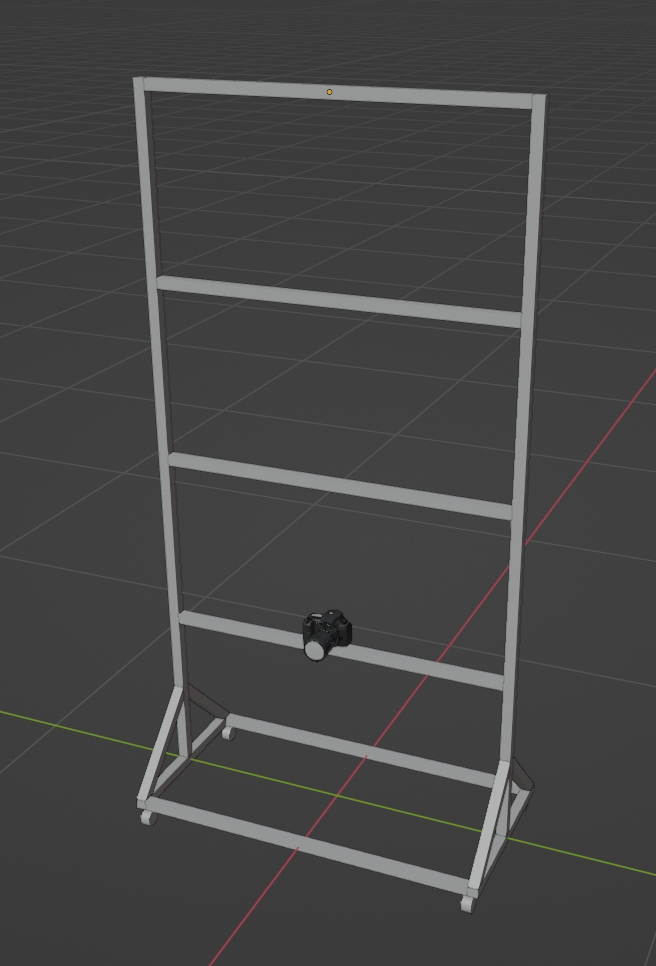
\includegraphics[height=5cm]{figures/frame-design}
    \caption{设计图}
\end{subfigure}%
\begin{subfigure}[b]{0.47\textwidth}
    \centering
    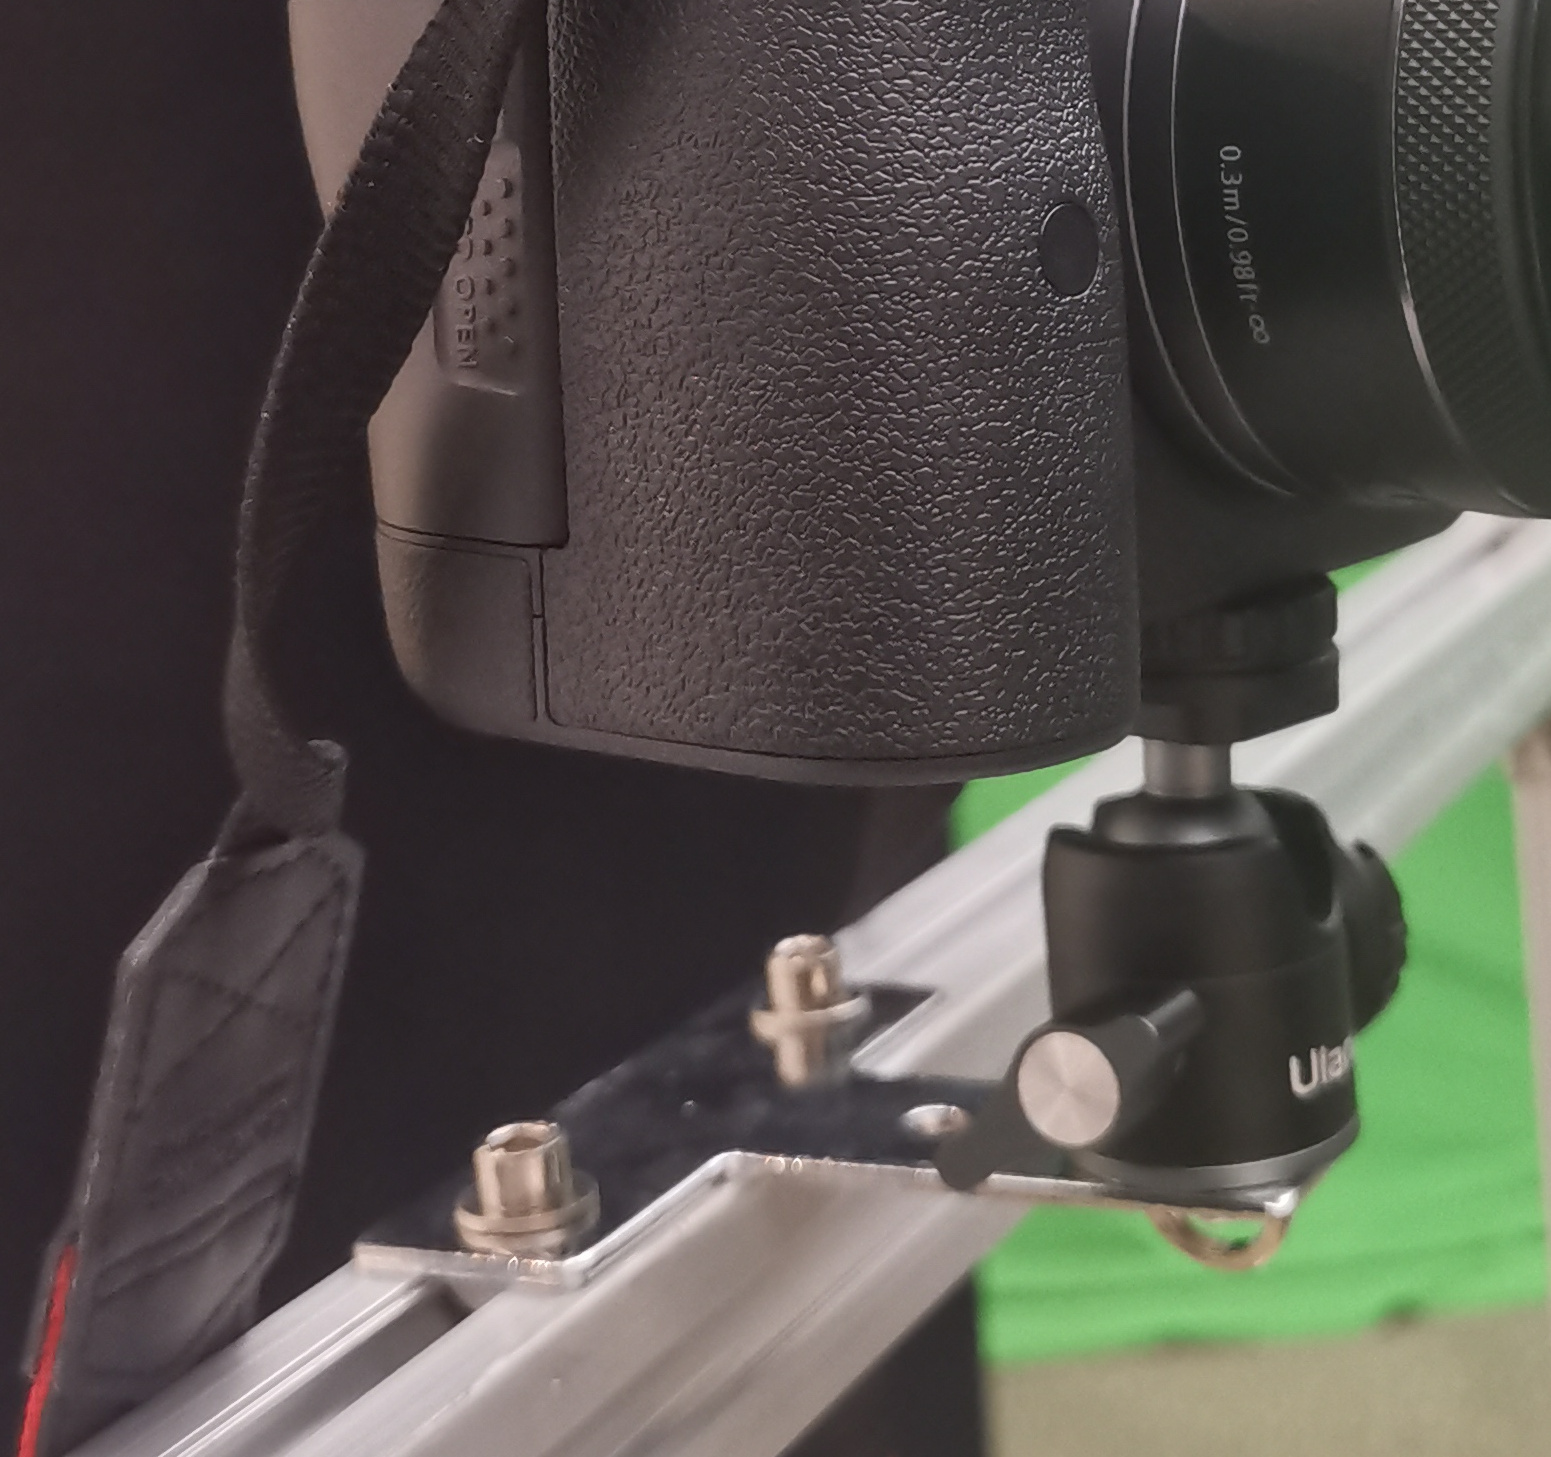
\includegraphics[height=5cm]{figures/frame-camera}
    \caption{相机固定}
\end{subfigure}
\caption{铝型材支架的设计和实现}
\label{fig:frame}
\end{figure}
如图\ref{fig:frame}所示。本系统相机固定在3个铝型材搭建的、定制的、高自由度可调节的支架上。
单个支架的主体部分由4个2寸脚轮,12.47米3030铝型材以及若干连接件组成。
设计全高2.103米,长1.06米,宽0.53米。
其物料成本约需要700元。
考虑到实验场地可能的变动,支架装配有4个脚轮,方便移动,且这些脚轮带有锁定功能,在使用时也能固定支架的位置。
脚轮固定在矩形底座上,底座则通过大量连接件,尽可能稳固地支撑了两根2米长的竖直铝型材。
在竖杆之间设计有4根长1米的横杆。
每两根间设计间距为0.5米,但得益于本方案使用T型螺母固定,无需打孔,因此这些横杆的位置可根据需要随时调整。

相机可固定在任意竖杆和横杆上的任意位置。
为固定相机,本方案首先将T型连接板通过T型螺母固定在铝型材上,然后将一个球形云台通过1/4英寸螺栓固定在连接板上,最后将相机通过标准的1/4英寸接口固定在云台上。
使用云台可允许相机以三个自由度任意旋转,再加上相机固定位置,横杆位置,以及支架整体的移动,相机最终固定位置的可调节自由度非常高。

\section{相机被动同步}

本方案使用的是12台消费级微单相机,型号为佳能R6。
被动同步旨在使它们精确地在同一时刻触发快门,以确保后期重建过程不会受到被拍摄对象的位移或形变影响。
该装置构造简单,且无须独立供电。
它通过2.5mm快门线接口控制相机的对焦和快门。

\begin{figure}
    \centering
    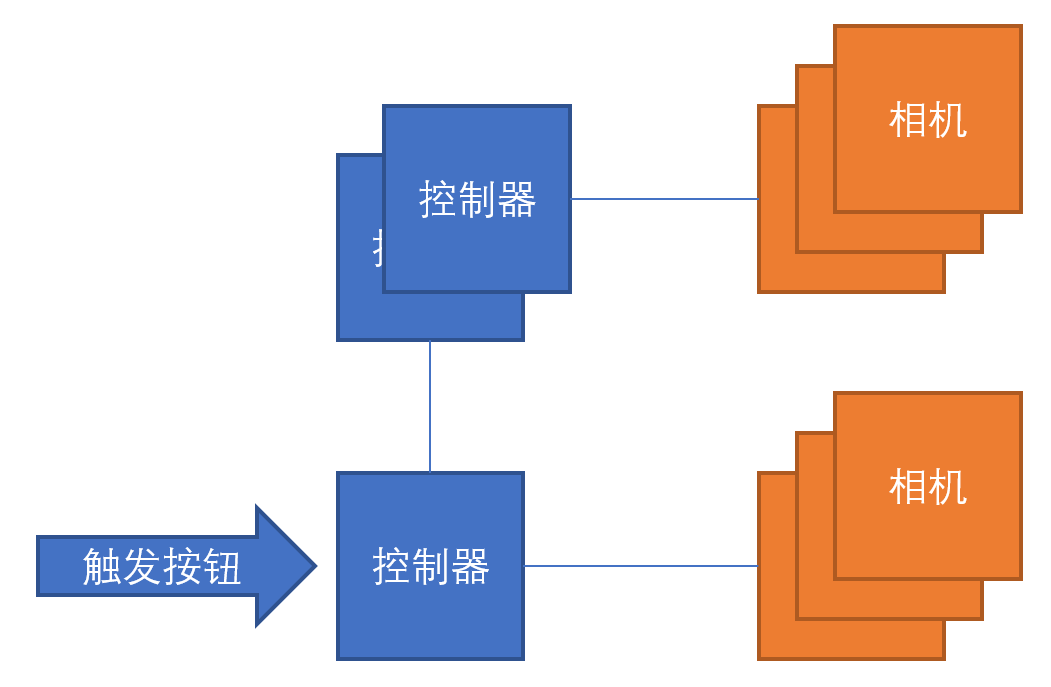
\includegraphics[height=5cm]{figures/passive_sync_topo}
    \caption{被动同步装置的拓扑结构}
    \label{fig:passive_sync_topo}
\end{figure}
如图\ref{fig:passive_sync_topo}所示,该装置可串联多个以扩展连接相机的数量。
\begin{figure}
    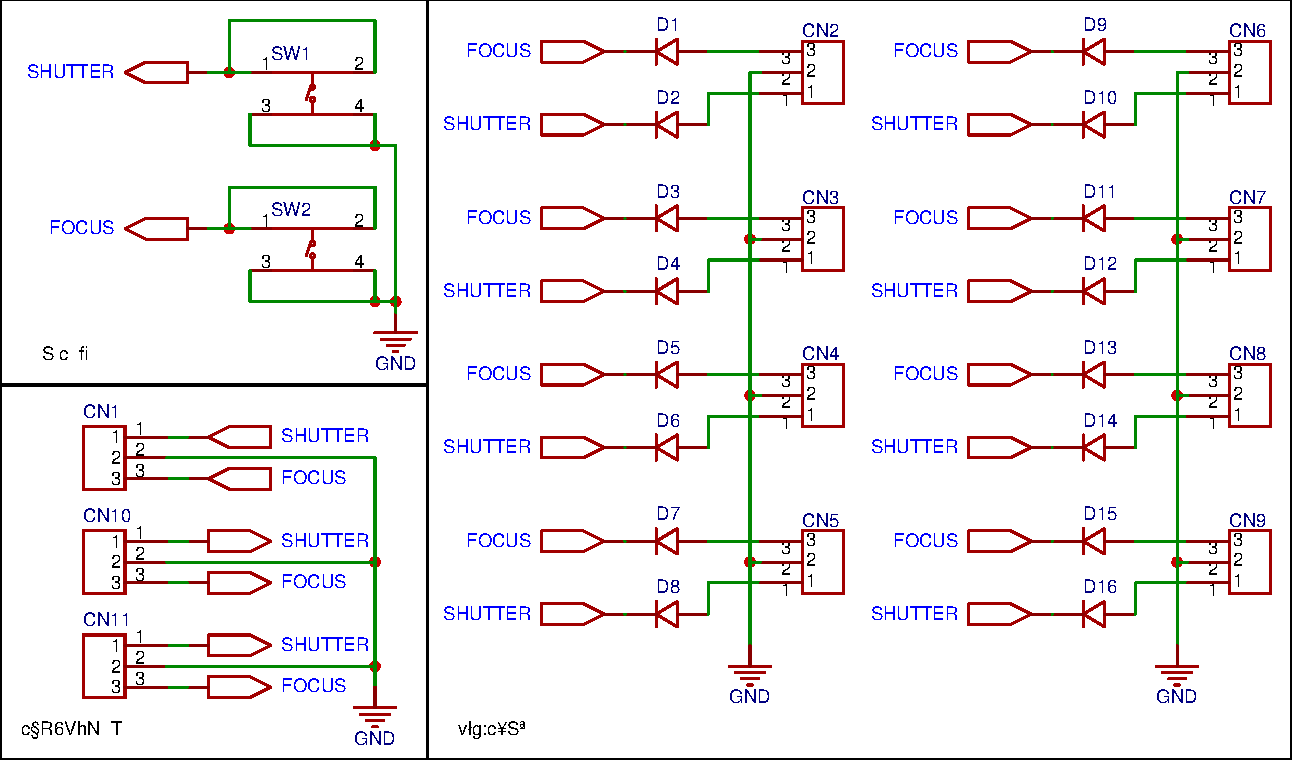
\includegraphics[width=\textwidth]{figures/passive_sync_schematic}
    \caption{被动控制器的电路原理图}
    \label{fig:passive_sync_schematic}
\end{figure}
其中,每个控制器的原理图如图\ref{fig:passive_sync_schematic}所示。
控制器无需供电,它采用机械按钮的形式完成控制线和底线的短接,从而触发相机快门。
控制器之间,以及相机与控制器间均采用AWG28规格的排线连接,
在控制器端均使用了冷压的XH2.54插头;
在相机段则使用了焊接的2.5mm插头。
此外,每个相机接口在连接到总线前均使用了两颗二极管进行隔离,以防止相机间的干扰。
这样可允许在控制器连接时依然可以手动控制单台相机的快门,也能防止在线缆连接时误触发快门。

\begin{figure}
    \centering
    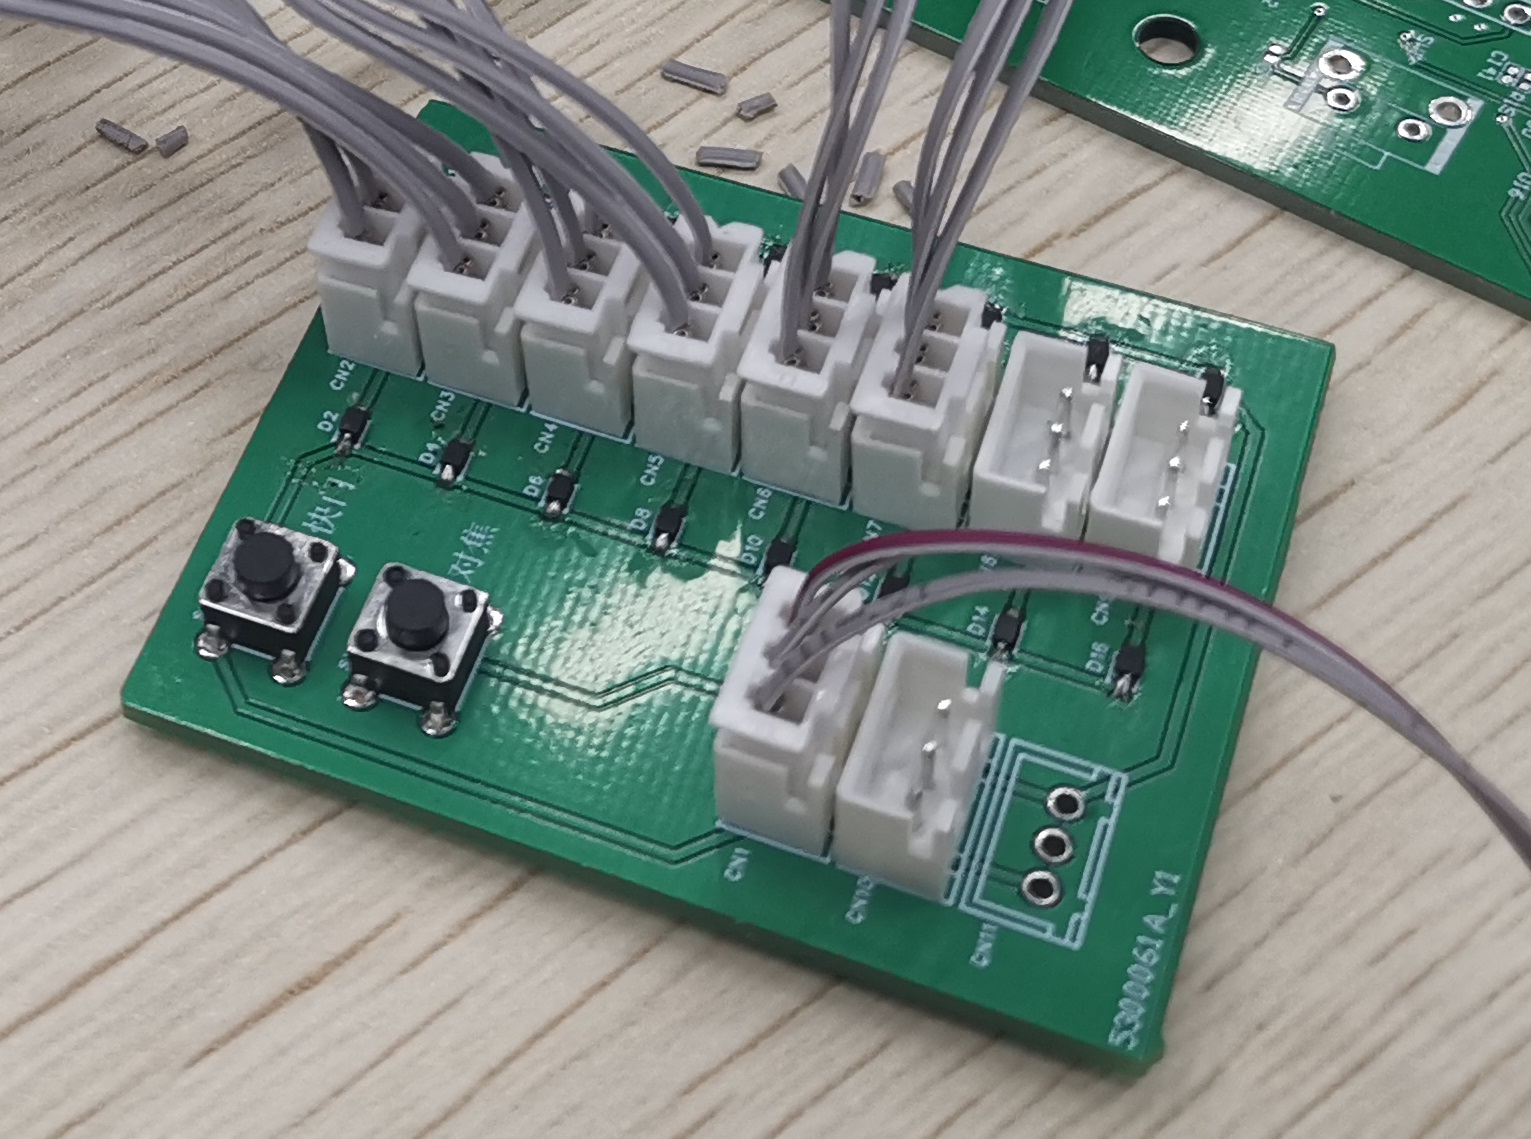
\includegraphics[height=8cm]{figures/passive_sync_controller}
    \caption{被动控制器的实物图}
\end{figure}

\section{相机/光源主动同步}

该装置带有一个单片机以完成可定制的实时控制,能独立控制每台相机、闪光灯触发延迟,最多可控制24台设备。
\begin{figure}
    \centering
    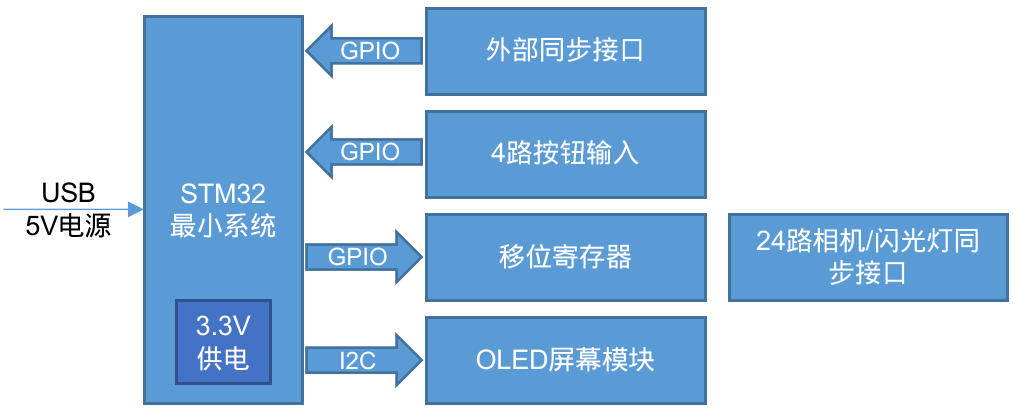
\includegraphics[width=0.8\linewidth]{figures/active_sync.png}
    \caption{主动同步装置硬件结构}
    \label{fig:active_sync}
\end{figure}
图\ref{fig:active_sync}展示了本方案中设计的主动同步装置的硬件结构。
该装置以一块STM32F103C8T6单片机为核心。
它通过GPIO接口,控制3块串联的74HC595D 8位移位寄存器,以控制最多24台相机或闪光灯,每个设备均通过XH2.54-3P插座与电路板连接。
作为系统指令输入和状态的反馈,该装置通过GPIO连接有4个机械按钮,可由软件指定其具体功能,并通过I2C总线连接了一个OLED显示屏模块。
此外,为了提升装置的可扩展性,还预留了一个用于外部同步的接口,可接收来自外部的对焦和快门触发同步信号,也连接到了单片机的GPIO接口,并通过XH2.54-3P插座暴露出来。

本装置采用移位寄存器是为了节省单片机的IO接口。
同时由于移位寄存器能通过单个电信号同时切换所有输出引脚的状态,这种设计也能实现更加精确的触发控制。
所采用的移位寄存器是富满FM生产的,该芯片输出引脚的功能与常见的推挽输出不同,它的输出引脚是开漏输出,
即当输出引脚为高电平时,该引脚呈高阻态,反之为低电平时,该引脚接地。
由于每个相机、闪光灯以及本控制器都是独立供电的,这种设计能起到一定的隔离作用,也能避免不同设备间由于电压不匹配造成的潜在问题。

\begin{figure}
    \centering
    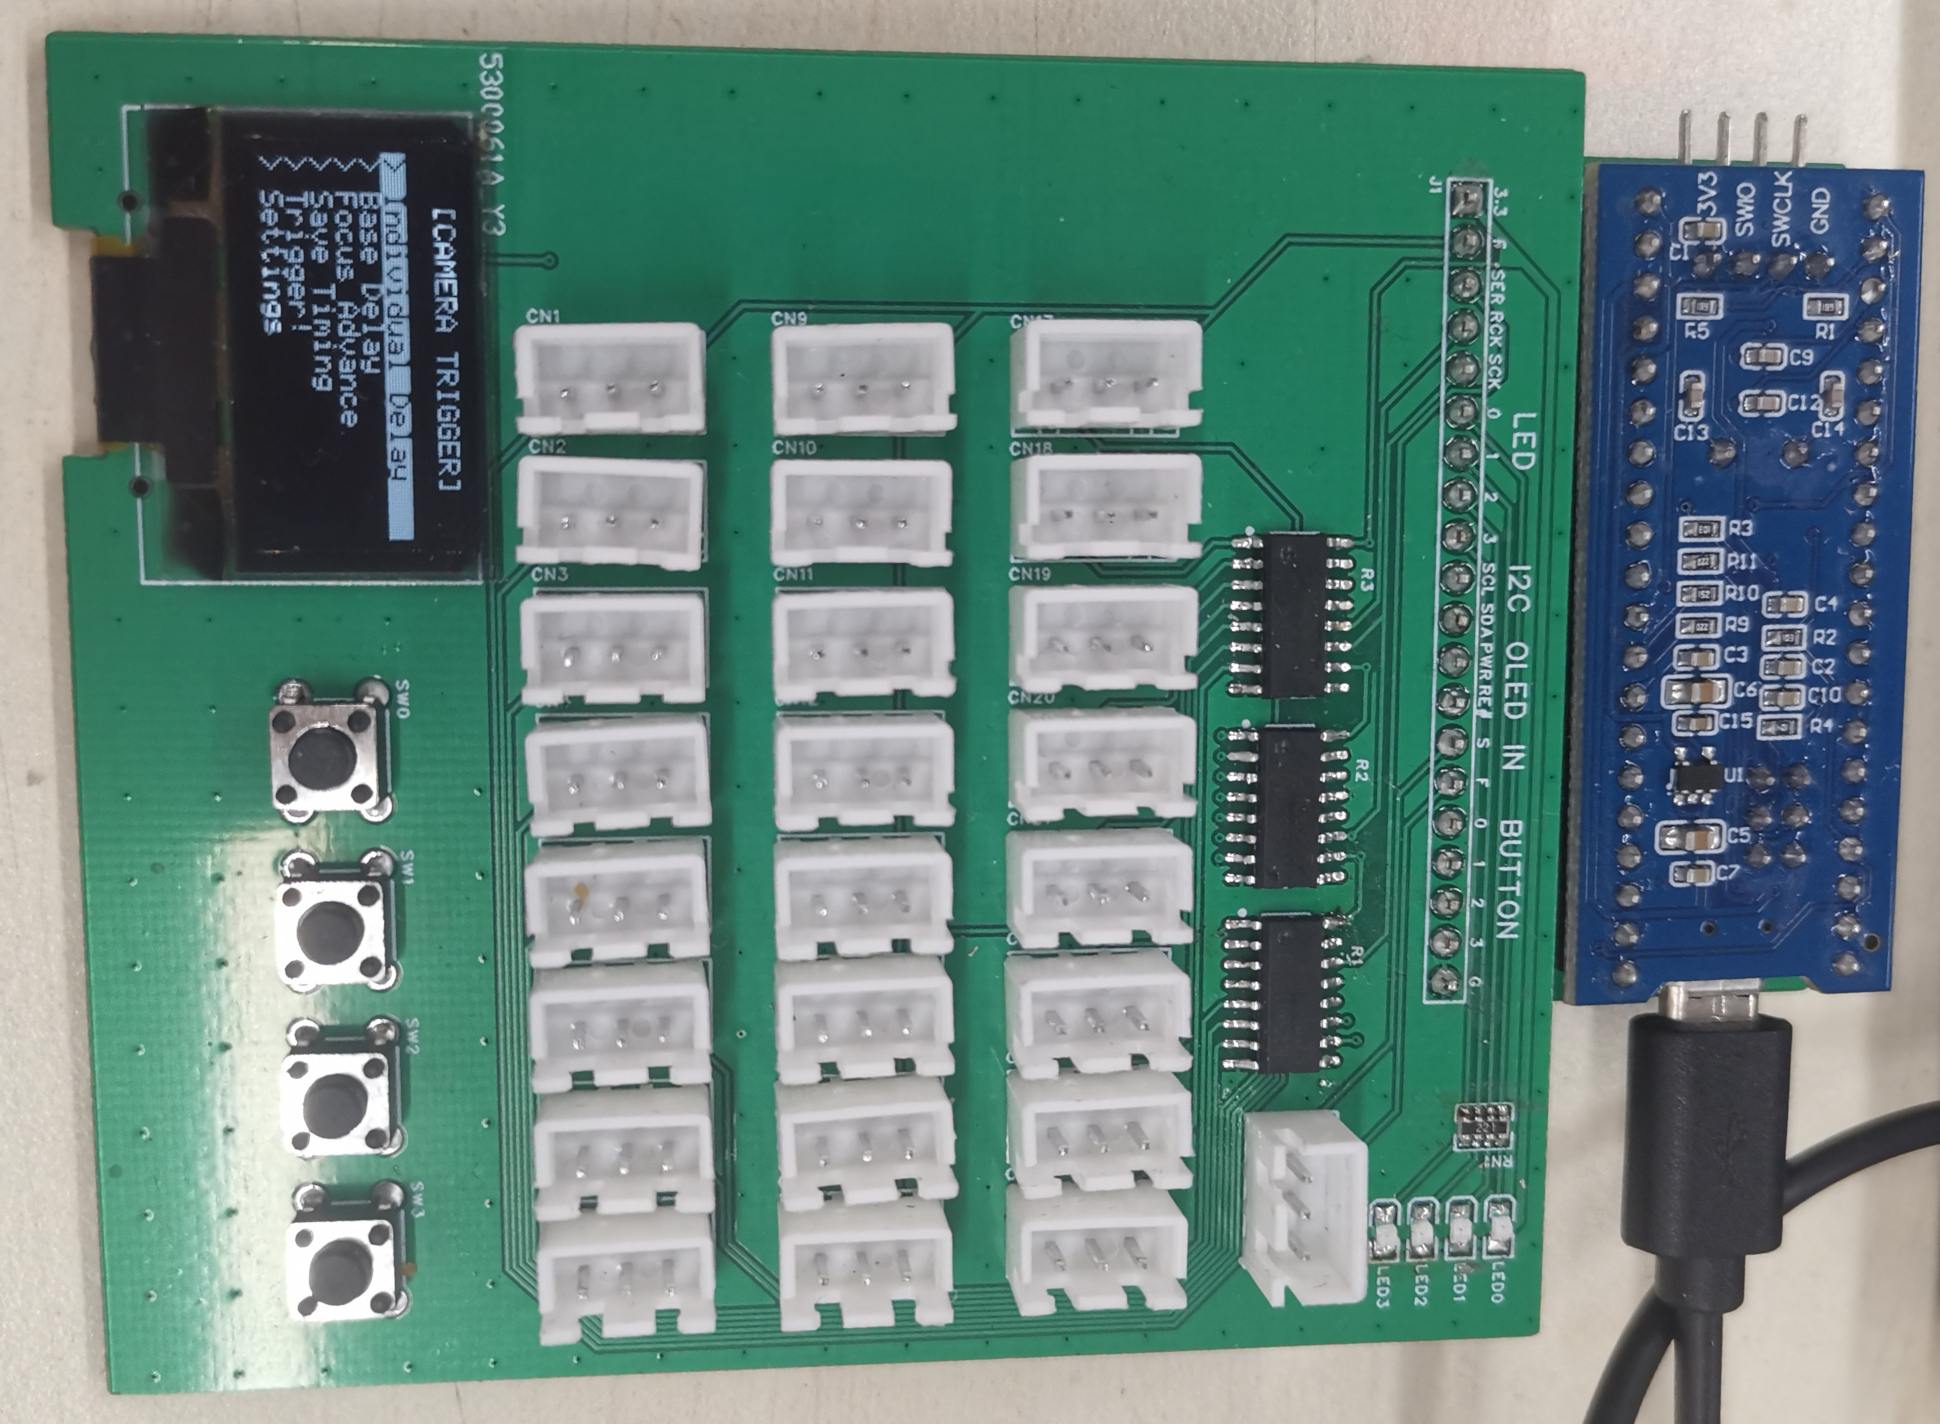
\includegraphics[width=\textwidth]{figures/active_sync_photo.jpg}
    \caption{主动同步装置实物照片}
    \label{fig:active_sync_photo}
\end{figure}

\begin{figure}
    \centering
    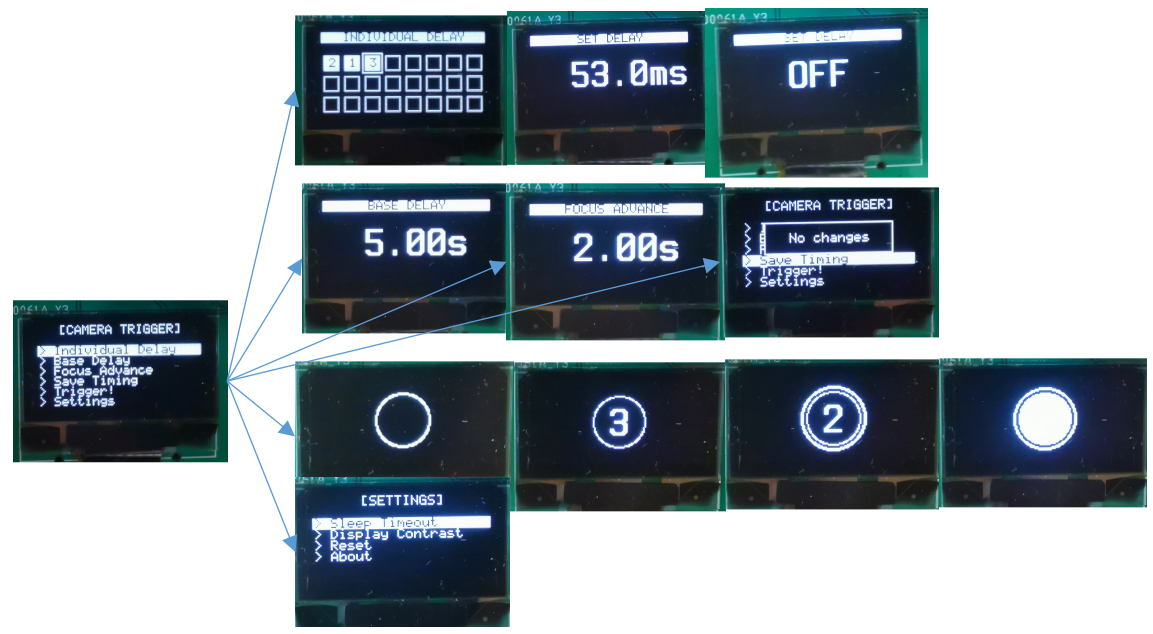
\includegraphics[width=\textwidth]{figures/active_sync_ui}
    \caption{主动同步装置用户界面}
    \label{fig:active_sync_ui}
\end{figure}
图\ref{fig:active_sync_ui}展示了该装置具体的配置选项设置和用户界面设计。
在菜单的导航中,从左到右四个按钮的功能设置分别为:上一项,确认,下一项,返回;
在数值设置界面,这些按钮则分别为:减小,切换开启/关闭,增大,确认。
在各设备延迟设置界面,用户可查看每个设备的触发顺序,并可分别设置每个设备是否触发,以及触发的延迟。
用户还能设置整体的触发延迟,以及在触发快门前需要提前多久触发对焦操作。
同时,用户可将这些时序设置保存到单片机的内置flash中,以便在下次上电时自动加载。
在快门触发界面,用户可按确认按钮开始触发流程,此时屏幕将显示倒计时,在触发对焦时显示一个额外的同心圆。
倒计时结束后,屏幕将显示实心圆,设备将进入高精度定时模式,并以设定的时序触发各个设备。
最后,在系统设置界面,用户可以配置显示器的亮度,进入睡眠状态的延迟,恢复出厂设置,以及查看当前软件的版本信息。
系统设置同样可以持久化到flash中。

\section{照片拷贝和整理}

在完成所有采集后,需要将所有照片拷贝到计算机上,整理以供后续算法使用。
本系统尝试了使用相机内建的Wi-Fi功能进行自动化,但链接速度过于缓慢,最终没有采用。
于是本方案最终使用了半自动化的方式。
如图\ref{fig:copy_photo}所示,
在计算机中运行一个自动拷贝进程,它利用Linux的udev系统监听SD卡连接计算机的事件。
利用该程序,手工从相机中取出SD卡后,只需将卡插入读卡器,程序便会自动完成挂载、拷贝、卸载的过程,之后需在提示时手工拔出并换入下一张卡。全程无需对计算机进行任何操作。
\begin{figure}[htb]
\centering
\begin{tikzpicture}
    \node [rectangle,draw=black,rounded corners=3mm] (start) {进程启动};
    \node [rectangle,draw=black] (wait) [right=of start] {等待SD卡插入};
    \node [rectangle,draw=black] (mount) [right=of wait] {挂载SD卡};
    \node [rectangle,draw=black] (copy) [right=of mount] {拷贝照片};
    \node [rectangle,draw=black] (unmount) [below=of mount] {卸载SD卡};
    \node (manual) [below=of wait] {手动插入下一张卡};

    \path [->] (start) edge node {} (wait)
        (wait) edge node {} (mount)
        (mount) edge node {} (copy)
        (copy) edge node {} (unmount)
        (unmount) edge node {} (wait)
        (manual) edge node {} (wait);
\end{tikzpicture}
\caption{半自动照片拷贝进程流程图}
\label{fig:copy_photo}
\end{figure}

然后,在计算机中需要人工对大量拍摄的照片进行筛选、分类,以去除不符合标准的照片,并将不同照片送入不同的下游流程处理。
\begin{figure}
\centering
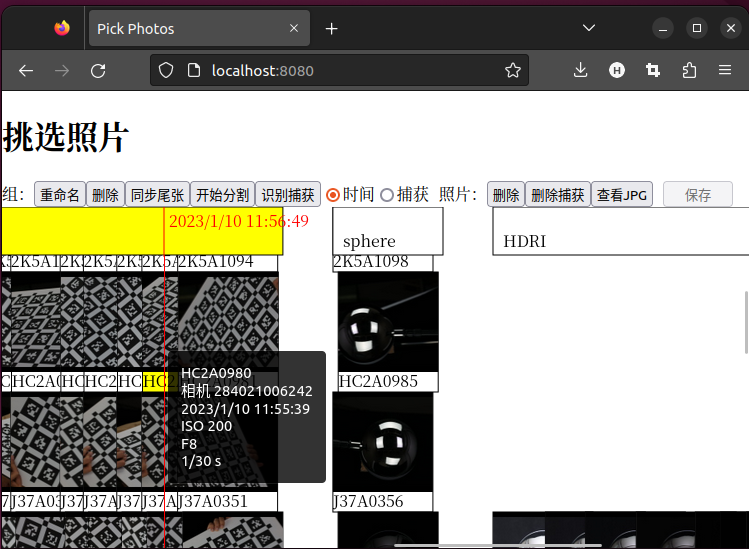
\includegraphics[width=\textwidth]{figures/pick_photo}
\caption{照片整理工具UI截图}
\label{fig:pick_photo}
\end{figure}
为此,本方案中包含了一个基于Web的照片整理工具。其界面如图\ref{fig:pick_photo}所示。
该工具可以快速从CR3格式的照片中提取预览图和高分辨率的预览JPEG图,以便于快速浏览。
该工具可以识别拍摄相机的序列号,将同一台相机的照片放在一行。并利用照片中记录的时间戳信息,将照片按照时间顺序排列,并根据时间间隔自动分组。
然后,用户可根据需要对组进行重命名、删除、拆分等操作。
用户也可以删除单张照片,或单次快门的所有照片。
此外,本工具还包含了一个基于贪婪算法的快门匹配程序,用于自动匹配同一次快门的所有不同相机拍摄的照片,并可输入后续的相机标定等算法。
该工具基于Web技术开发还有一个额外的好处,用户可以在任意终端上完成整理工作,而不需要在本地安装任何软件,也不需要在本地拷贝大量的照片数据。

\section{相机标定}

本系统选用的相机模型是针孔相机模型,这也是在实验中采用的相机所遵循的模型。
由于本实验中相机畸变较小,简单起见,本系统选用了OpenCV中默认的径向和切向相机畸变模型\footnote{https://docs.opencv.org/4.7.0/d4/d94/tutorial\_camera\_calibration.html}。

\begin{figure}
    \centering
    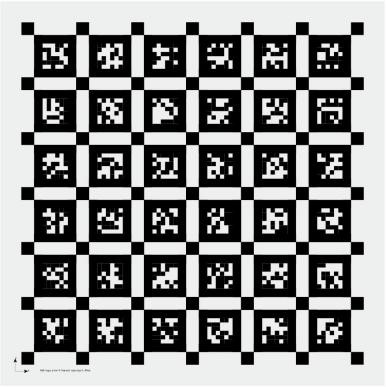
\includegraphics[width=0.5\textwidth]{figures/april_board}
    \caption{April Board上印制的二维码和棋盘格图案}
    \label{fig:april_board}
\end{figure}
本系统中使用的标定物体为April Board,即印有二维码和棋盘格组成的图案的标定板,如图\ref{fig:april_board}所示。
该标定板的尺寸为$800 \times 800$毫米,每个二维码的边长为$88$毫米。

\begin{figure}[htb]
\centering
\begin{tikzpicture}
    \node [rectangle,draw=black] (init) {内参初始化};
    \node [rectangle,draw=black] (stage1) [right=of init] {每相机独立标定};
    \node [rectangle,draw=black] (transfer) [right=of stage1] {外参传递};
    \node [rectangle,draw=black] (ba) [right=of mount] {集束调整};

    \path [->] (init) edge node {} (stage1)
        (stage1) edge node {} (transfer)
        (transfer) edge node {} (ba);
\end{tikzpicture}
\caption{相机标定流程图}
\label{fig:calib_proc}
\end{figure}
本系统中的相机标定流程如图\ref{fig:calib_proc}所示。
\begin{figure}
\centering
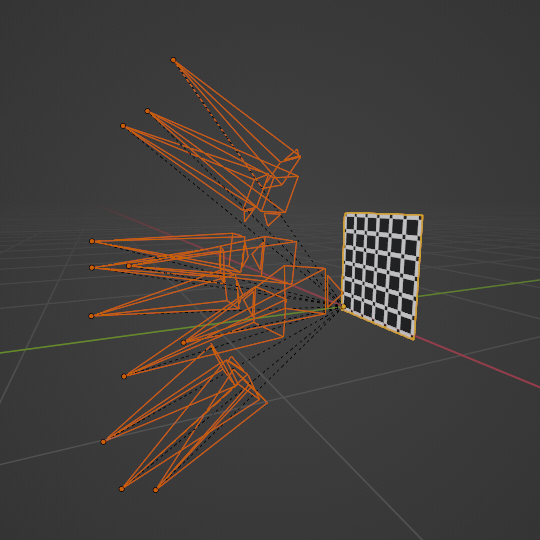
\includegraphics[width=0.8\textwidth]{figures/calib_vis}
\caption{导入到Blender中的相机标定结果可视化}
\label{fig:calib_vis}
\end{figure}
标定结果如图\ref{fig:calib_vis}所示。

\section{环境光照标定和HDRI合成}

该步骤的目的是将上述拍摄的多张照片中各自最可靠的部分(信噪比高,且未超出传感器量程范围)融合为一张HDRI。
为此,本文设计了一种类似卡尔曼滤波的融合算法。
其基本思想是:将不同照片中的同一像素点的读数视为对同一光照强度的不同测量值,并有不同的测量噪声方差,据此对多个观测值加权平均,得到最可能接近真值的估计值。

但我们仍然需要一种方法将环境光照的方向映射到该照片中的像素坐标上,以便于在渲染时使用。
该映射取决于诸多因素,如用于拍摄的相机的内外参,球在照片中的位置等。
\begin{figure}
    \centering
    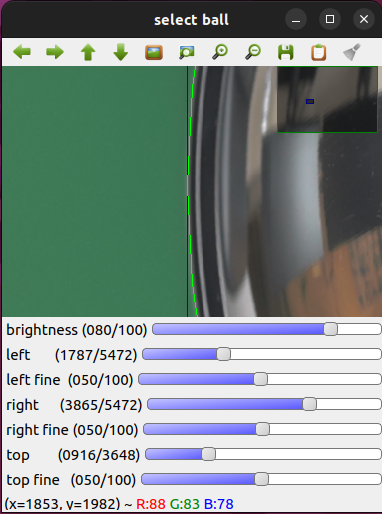
\includegraphics[height=8cm]{figures/sphere_locator}
    \caption[反射球位置标注工具界面]{反射球位置标注工具界面。上半部分中蓝色线为当前指定左平面位置,绿色为解算出的反射球位置重投影回像素空间的轮廓}
    \label{fig:sphere_locator}
\end{figure}
首先,为了准确得到反射球在照片中的位置,本方案开发了一款标注工具以允许用户手动选中球的位置,如图\ref{fig:sphere_locator}所示。
该工具在上部将显示经过畸变校正的照片,用户可以自由缩放和平移,以及改变照片的亮度以便观察。在照片上叠加显示了当前选中的球位置的轮廓。
在下部显示了三组滑块,分别用于调整轮廓的左边界、右边界和上边界在照片中的位置。每组滑块分为粗调和细调两部分,细条滑块允许用户在粗调结果周围10像素进一步细化结果。
需要注意的是,这里显示的球的轮廓虽然很接近,但并不是一个圆形。为了尽可能精确,本文将解算后球的位置按照标定的参数重新投影到照片上,进而获取该轮廓。

为了得到可直接在下游任务中使用的环境光照贴图,本方案在照片中反射球所在区域的每个像素处生成一个顶点,并将其连接成三角形网格,从其像素坐标计算每个顶点的纹理坐标,并按照计算的光照方向将其放置在3D单位球上的对应位置,然后使用OpenGL对所生成的网格进行光栅化渲染,在片元着色器中根据纹理坐标对HDRI采样。
根据所需环境光照贴图的格式不同,可使用不同的顶点着色器完成对应的顶点坐标变换。
本项目已支持常见的等距柱状投影(Blender中使用)和立方体贴图(nvdiffrast中使用)两种格式。
\begin{figure}
    \begin{tikzpicture}
        \node [inner sep=0pt, anchor=north west] at (0,0) {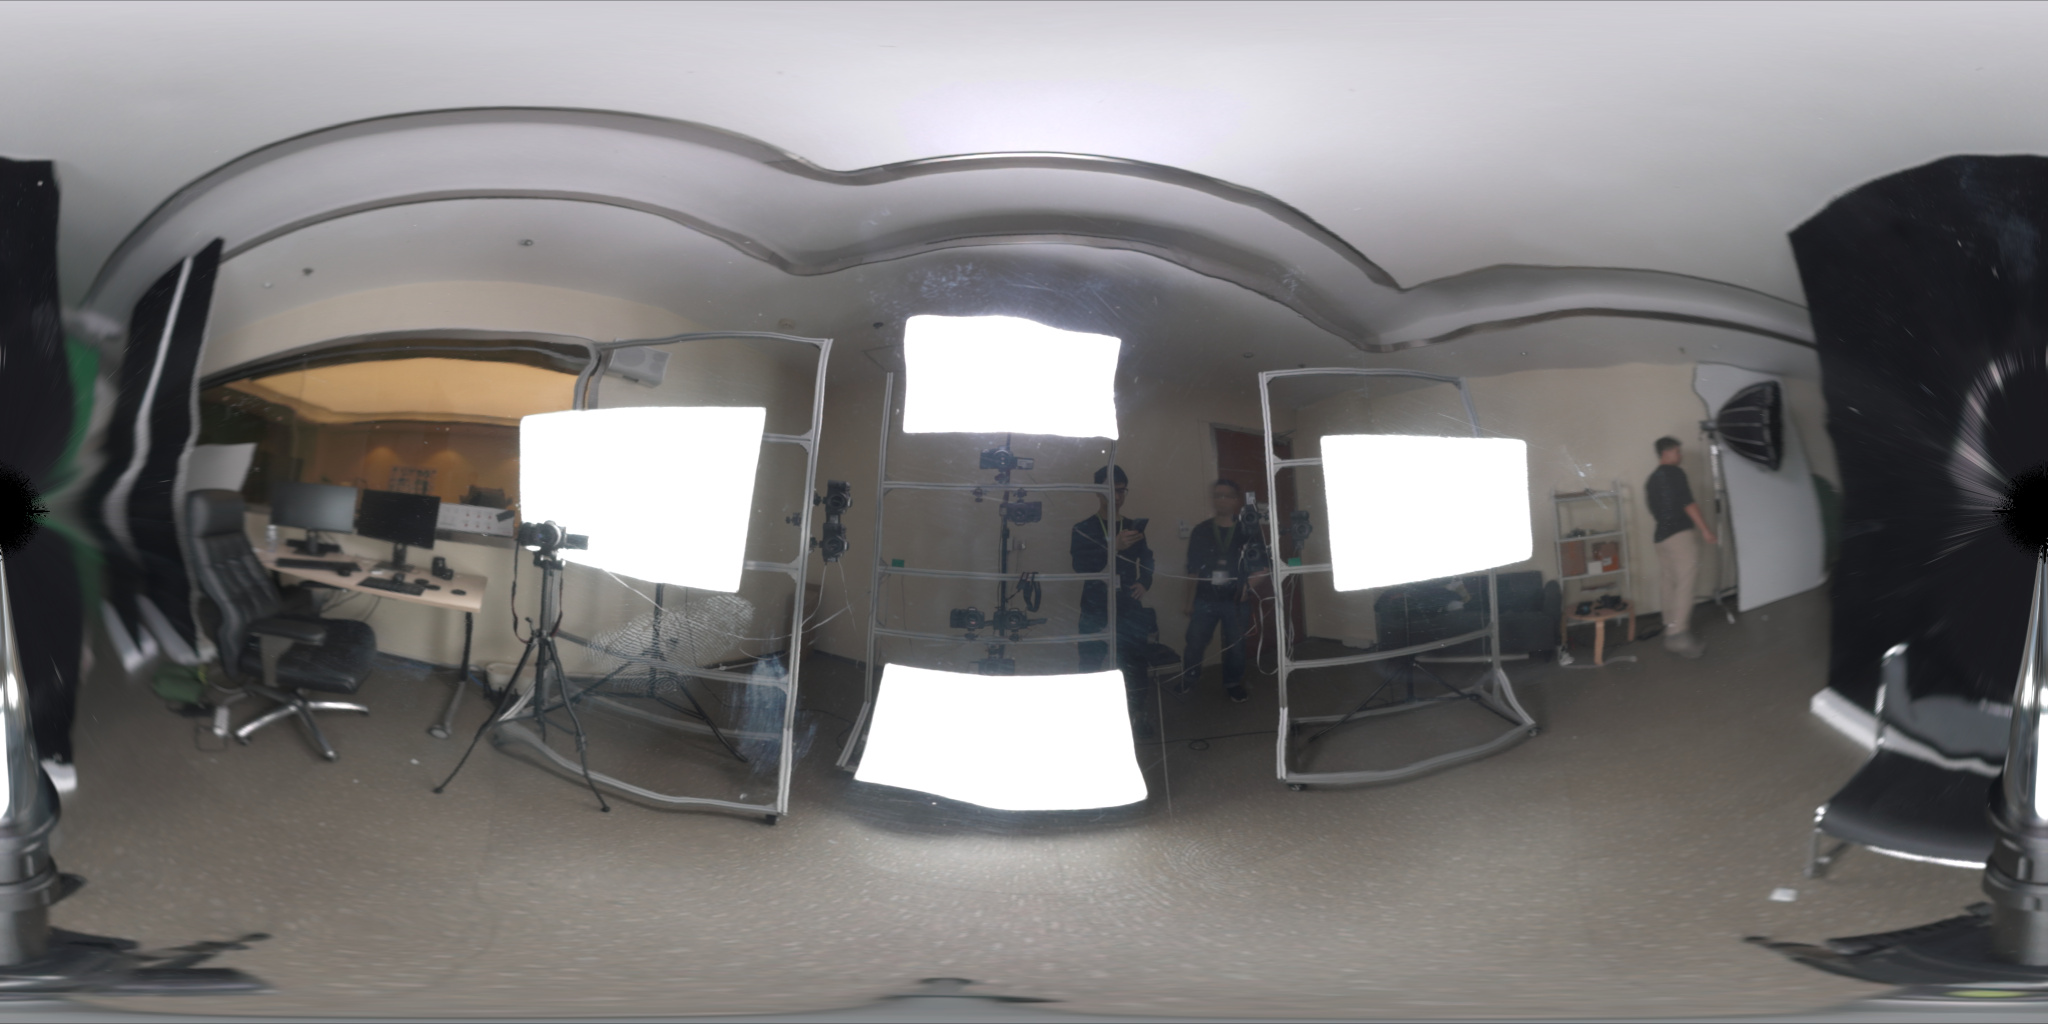
\includegraphics[width=\textwidth]{figures/HDRI}};

        \def\w{4096}
        \node [inner sep=0pt, anchor=north west] (part) at (6.5cm,-0.5cm) {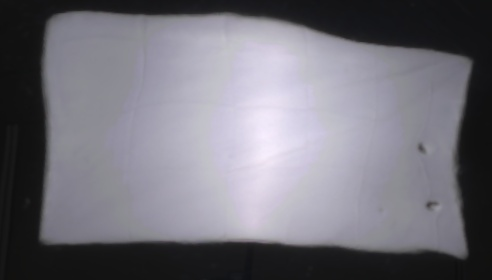
\includegraphics[width=0.1201171875\textwidth]{figures/HDRI_light_part}};
        \coordinate (a) at ({(1768/\w)*\textwidth},{(-620/\w)*\textwidth});
        \coordinate (b) at ({(2260/\w)*\textwidth},{(-900/\w)*\textwidth});
        \node [inner sep=0pt, anchor=north west, draw=red, fit=(a) (b)] (light) {};

        \path [->] (light) edge [red] node [left] {/32} (part);

    \end{tikzpicture}
    \caption[实验环境全景HDRI]{实验环境全景HDRI。通过多张金属反射球的照片合成。大图中展示了其中较暗部分的信息,小图展示了其中一个柔光箱处亮度调整到1/32时的图像}
    \label{fig:HDRI}
\end{figure}
图\ref{fig:HDRI}即为使用本方案生成的等距柱状投影格式的环境光照贴图。

\end{document}
